\documentclass[10pt,letterpaper]{article}

\usepackage{cogsci}
\usepackage{pslatex}
\usepackage{apacite}
\usepackage{graphicx}
\usepackage{amsmath}
\usepackage{amsfonts}
\AtBeginDocument{\RequirePackage{lmodern, times}}

\newcommand{\argmax}[1]{\underset{#1}{\text{argmax}}\ }

\title{One-shot learning of generative speech concepts}
 
\author{Authors}
 
%\author{{\large \bf Morton Ann Gernsbacher (MAG@Macc.Wisc.Edu)} \\
%  Department of Psychology, 1202 W. Johnson Street \\
%  Madison, WI 53706 USA
%  \AND {\large \bf Sharon J. Derry (SDJ@Macc.Wisc.Edu)} \\
%  Department of Educational Psychology, 1025 W. Johnson Street \\
%  Madison, WI 53706 USA}

\begin{document}
\maketitle

\begin{abstract}
\textbf{Keywords:}
speech recognition; category learning; one-shot learning; exemplar generation
\end{abstract}

\section{Introduction}
There has been recent interest in one-shot learning -- the human ability to learn a new concept from just one or a few examples \cite<e.g.,>{CareyBartlett1978,Markman1989,Ahn1992,Xu2007}. Although one-shot learning is an important aspect of everyday cognition, traditional learning algorithms can require tens, hundreds, or thousands of examples before reaching a high level of classification performance. This mismatch poses a challenge to computational approaches for understanding human-level concept learning, yet over the last several decades, the fields of cognitive science and machine learning have made significant progress. Cognitive models have sought to quantitatively explain the way people generalize from just just a few examples in a low-dimensional space \cite{Shepard1987,Feldman1997,Tenenbaum2001}. Other cognitive models and computer vision algorithms become better one-shot learners through ``transfer learning'' or ``learning to learn,'' where previous experience with related concepts helps to inform which dimensions or features are most important for generalization \cite{Bart2005,Colunga2005,FeiFeiFergus2006,KempPerfors2007}.

Despite real progress spanning multiple disciplines, we are still far from a satisfying computational account of one-shot learning. Previous models have been limited by the simplicity of the representations that they learn -- usually prototypes or exemplars in a feature space -- which lack the power necessary for capturing many types of natural concepts \cite{Murphy1985}. While these feature-based approaches can be useful for classification, they provide less insight into how background knowledge interacts with learning or how people generalize in other ways beyond classification, including exemplar generation \cite{Jern2013}, causal inference \cite{Rehder2003}, explanation \cite{Williams2010}, and conceptual combination \cite{Murphy1988}. Given that people learn very rich concepts, even from just one or a few examples, the central computational challenge is to explain how people extract so much information from such limited data.

Analysis-by-synthesis is the classic idea, beginning with Helmholtz, that sensory data can be more richly represented by modeling the causal process that generates it. This has been an influential approach to studying perception in vision \cite{Yuille2006} and speech \cite{Liberman1967}, where a perceptual classification decision can be made by selecting the category $c \in \{1,...,K\}$, defined by parameters $\psi_c$, that maximizes the probability of generating a data example $x^{(i)}$
\begin{equation}
\argmax{c} P(x^{(i)}|\psi_c).
\end{equation}
But learning is a more challenging problem, and there are good reasons to think an analysis-by-synthesis approach would not be successful for one-shot concept learning. Learning of a causal process from examples $x^{(1)},...,x^{(n)}$ can be formulated as the selection of a model $\psi_c$
\begin{equation}
\argmax{\psi_c} \prod_{i=1}^{n} P(x^{(i)} |\psi_c) P(\psi_c),
\end{equation}
from a potentially infinite space of possible models. Since this can be a very difficult problem and can require many training examples to achieve good generalization \cite<e.g.,>{Geman1992,HintonNair2006}, how could it possibly be learned from just a single training example? One-shot learning of generative models might only be sensible for a special subset of simple causal processes. If a human or machine was trying to learn what a ``tree'' was from just a single example, it would be hopeless to try to learn (or even represent) a fully-detailed process of biological growth, beginning with tree DNA and ending with the set of all possible trees. But at the right level of abstraction, the essence of a tree could be captured by a simple stochastic program, starting with a single branch and then recursively splitting until the tree terminates. With a prior $P(\psi_c)$ favoring simple generative processes, it seems possible to discover such a program from just a few examples.

What is the right notion of simplicity for formulating a prior over causal processes? Recent behavioral and computational work suggests that \emph{compositionality} may be key principle for both encouraging representational simplicity and transferring previously learned knowledge from related concepts \cite{Lake2012,Lake2013}. Freely combining primitive structure can be a powerful way to build complex object representations \cite{Biederman1987}, and when combined with ideas from Hierarchical Bayesian modeling \cite{Gelman2004}, it can also be a similarly powerful way to build a ``generative model for generative models'' that can perform one-shot learning. This idea was applied to the one-shot learning of handwritten character \cite{Lake2013}. Given a raw image of a new character, such as a character from a foreign alphabet, the model learns to represent it by a latent dynamic causal process, composed of pen strokes and their spatial relations (Fig. \ref{models}a). Sharing across characters is accomplished by the re-use of stochastic motor primitives (Fig. \ref{models}a-i) that can combine in new ways to make new characters (Fig. \ref{models}a-iv). From just a single example, this model could both classify and generate new  examples at a human level of performance.

\begin{figure*}[t]
\centering
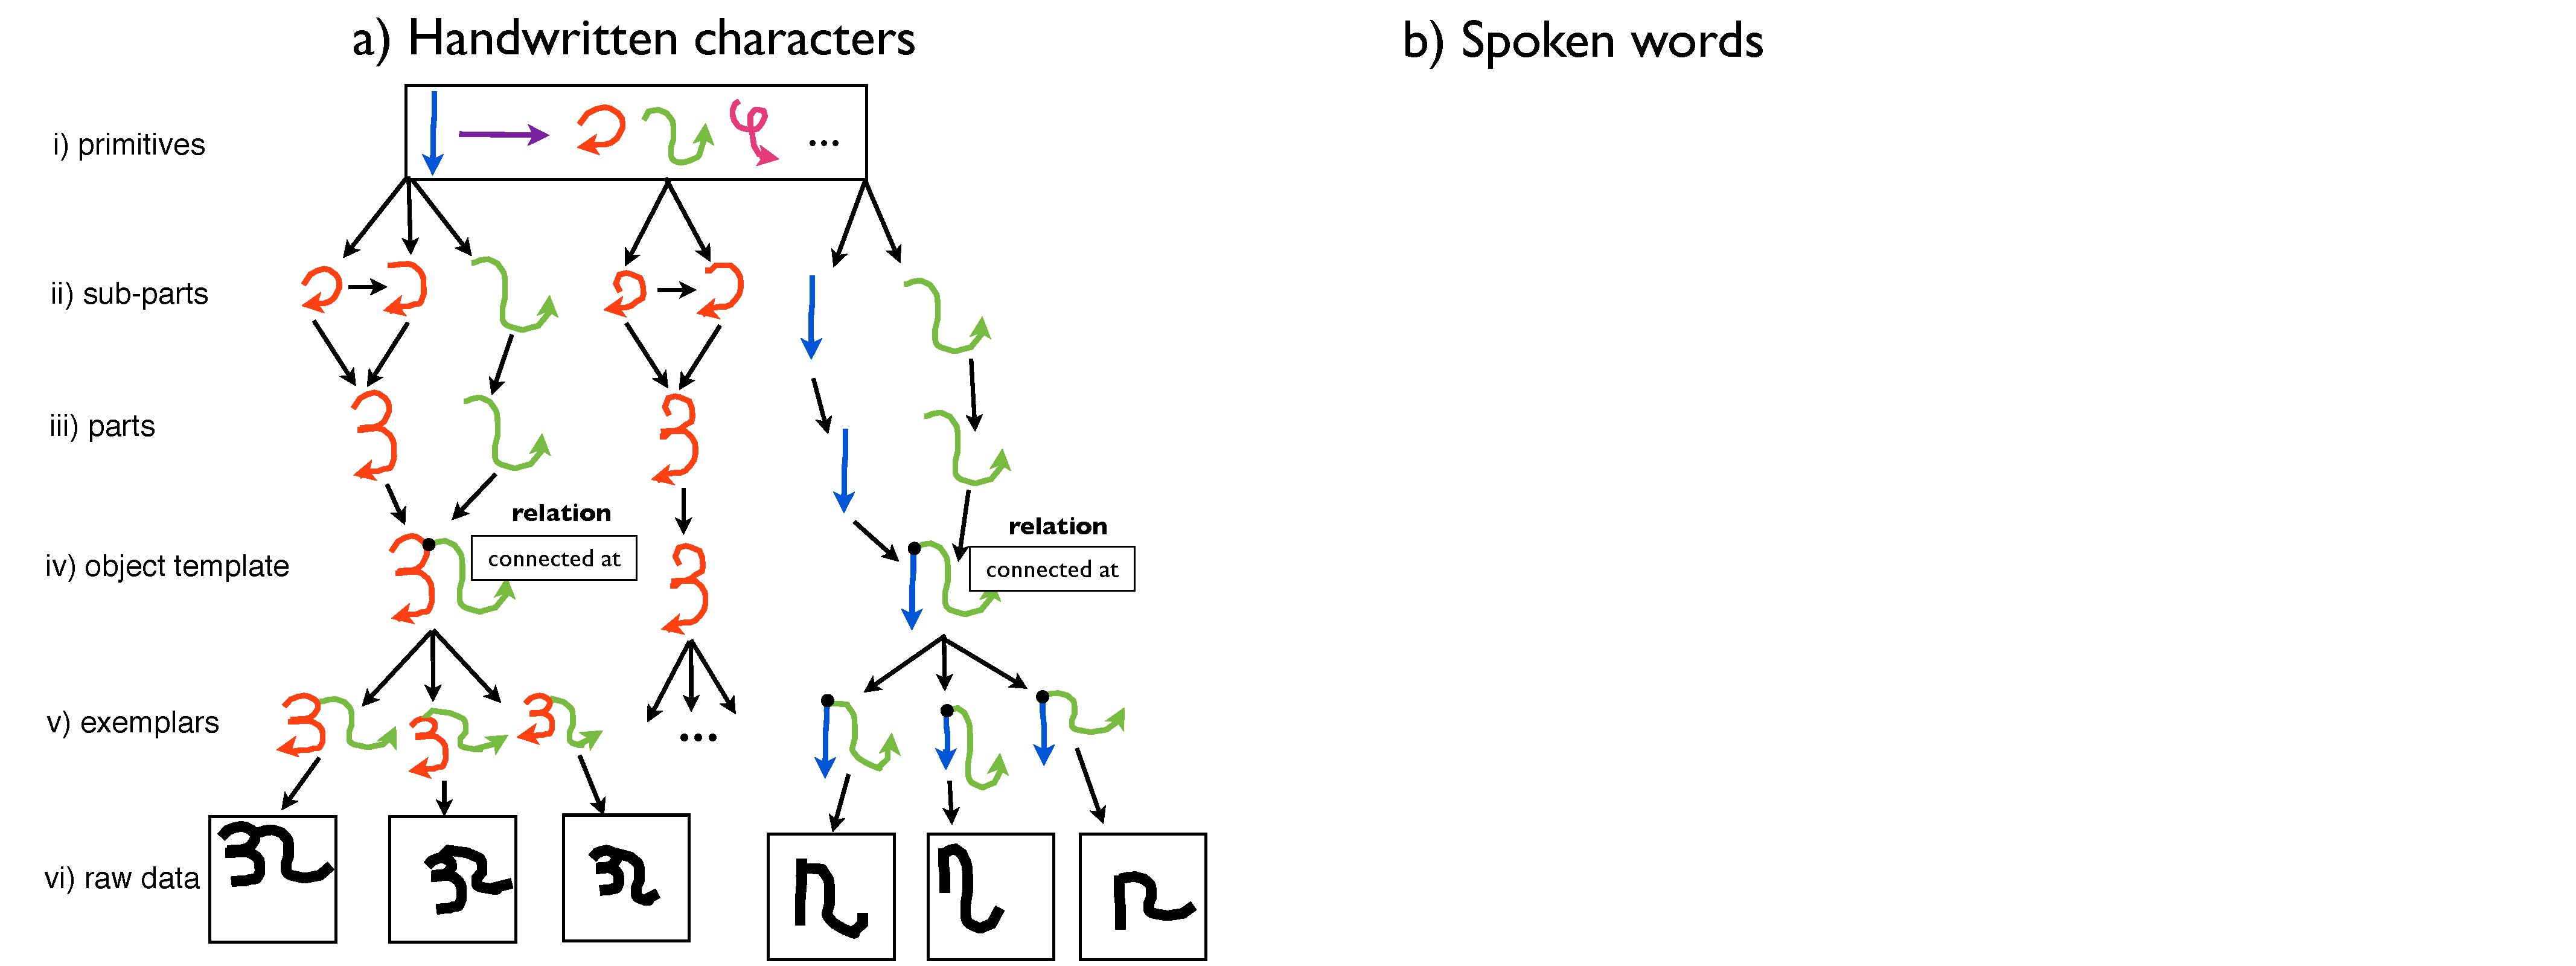
\includegraphics[width=7in]{model.pdf}
\caption{Hierarchical Bayesian modeling as applied to handwritten characters and speech.}
\label{models}
\end{figure*}

How general is this approach, and could it apply to learning non-visual concepts? In this paper, we extend these ideas to the one-shot learning of new spoken words, such as a young child learning to recognize and pronounce a new word (the speech sound for ``elephant'') or an adult learning a word in a foreign language (like the word ``elephant'' in Japanese). Speech is a promising domain for our approach, since analysis-by-synthesis has been influential in speech recognition for decades \cite{Halle1962,Liberman1967} and there is a clear compositional structure of phonemes that could be exploited for learning. From the raw speech signal of a word, our model infers a causal representation based on a sequence of phone-like units (Fig. \ref{models}b). Like the characters, the prior distribution on these sequences are learned from experience with other words and can be combined together in new ways to define a new word (Fig. \ref{models}b-iv). Since each inferred word representation is itself generative, it can be used to both classify new examples or generate new examples (Fig. \ref{models}a-v) from just a single instance of a new word. By transferring a prior on sub-unit sequences learned from a corpus of Japanese speech, the model can classify new Japanese words at a level of accuracy similar to English-speaking humans. We also compare humans and the model on another natural form of generalization -- an exemplar generation task.

\begin{itemize}
	\item Related work in ASR on open dictionary words
\end{itemize}

\section{Model}

\begin{itemize}
\item Describe general ASR approach, and how this is related (but unsupervised, like a child)
\item Mathematical description of the model
\end{itemize}

\section{Experiment 1: Classification}
People and several models were evaluated on a one-shot classification task using novel Japanese words. 

\subsubsection{Datasets.} 

\begin{itemize}
\item Discuss why Japanese?
\end{itemize}

\subsubsection{People.}
Participants were recruited on Amazon's Mechanical Turk from a population of individual in the USA. All analyses were restricted to native English speakers that do not know any Japanese, as reported in a post-experiment survey rather than as a qualification for participation. This population was used for this and all other experiments. 

Participants were asked to classify new Japanese words in a sequence of 10 (or 5) displays designed to minimize memory demands (Fig \ref{ss}). Each display had a set of buttons where each button played a sound clip of a Japanese word, with the``target word'' at the top and ``1'' through ``20'' beneath it. Each of the numbered buttons had an associated radio button for response selection. Participants were asked to pick the sound clip that produces the same word as the target word.

Participants had to pass an instructions quiz before beginning the experiment \cite{Crump2013}, and there was also a practice trial with English words. Sound clips could be played more than once, and responses were not accepted until all buttons had been tried. 

\begin{itemize}
\item Mention they never see the same word twice
\item Explain word lengths, etc. here or in stimulus section
\item explain two conditions (same vs. different gender)
\end{itemize}

\begin{figure}[h]
\centering
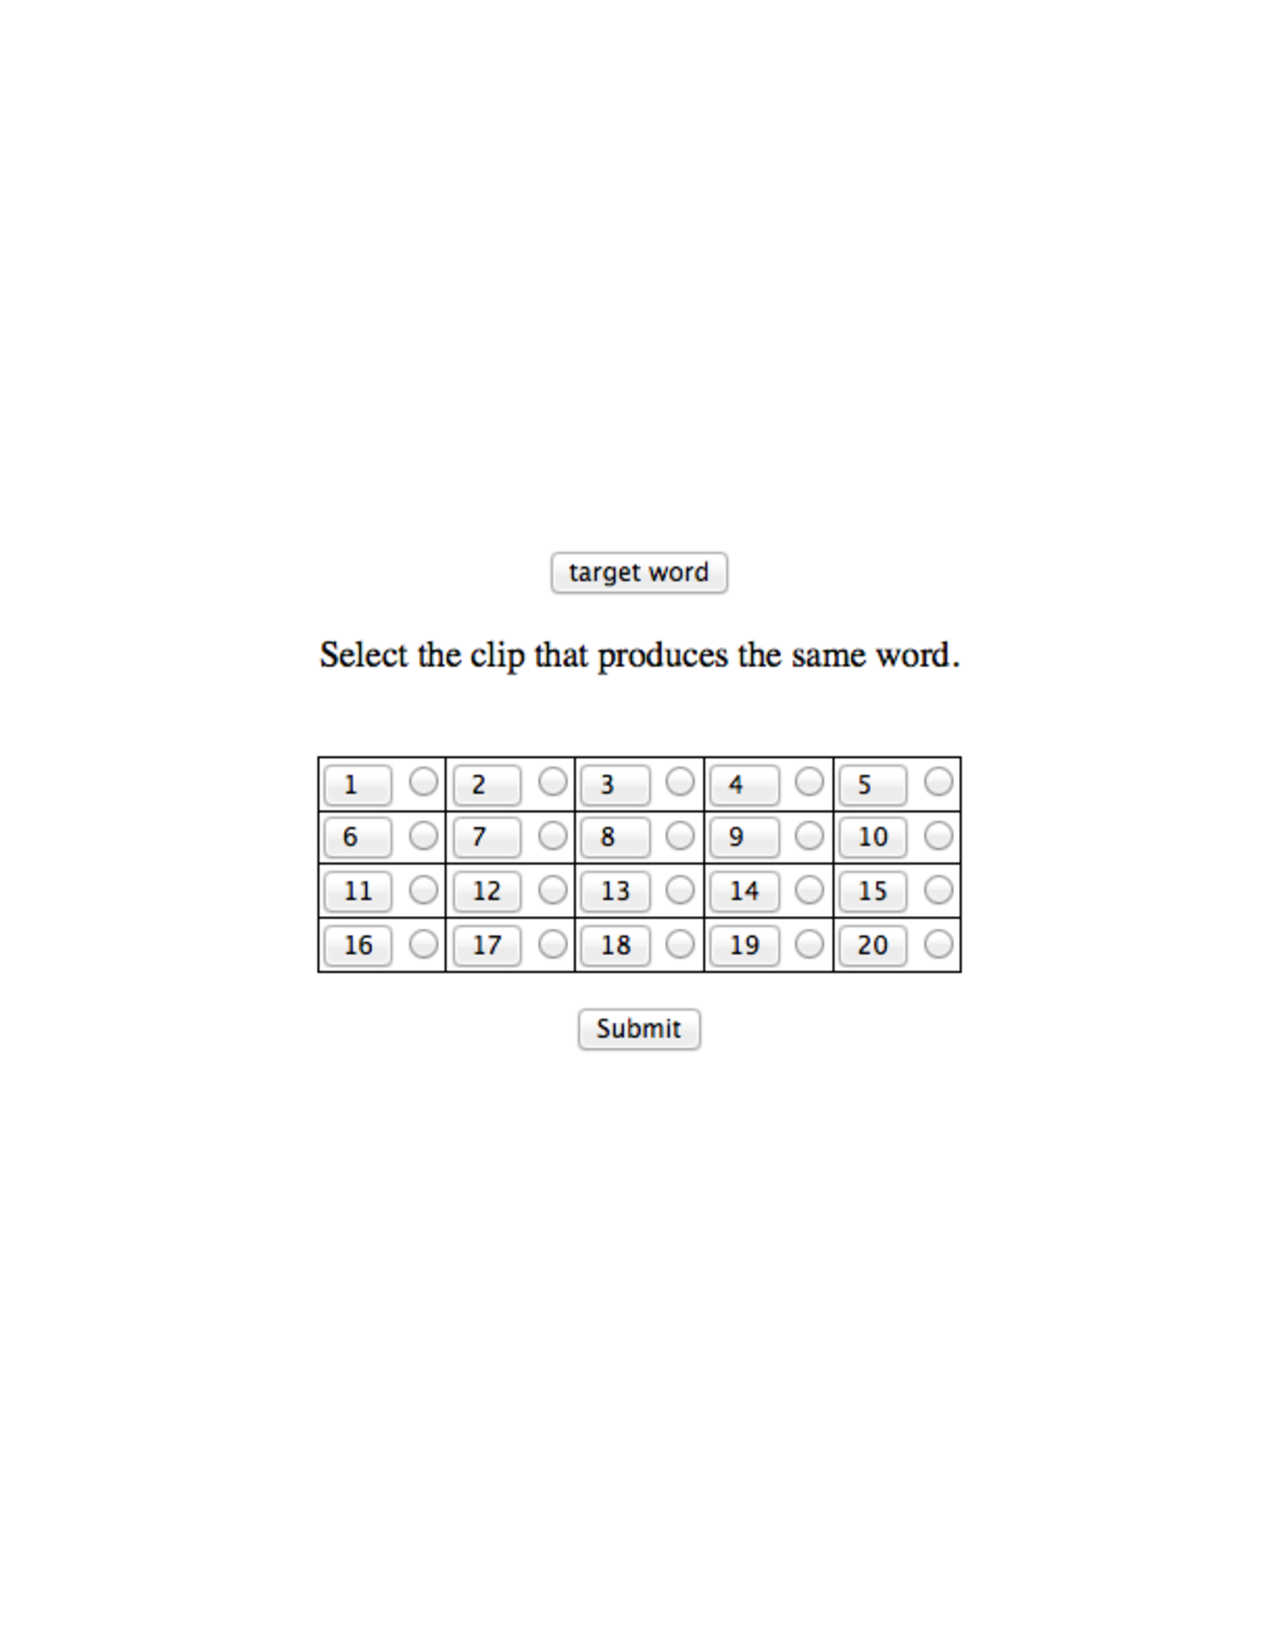
\includegraphics[width=2.25in]{web_exp.pdf}
\caption{Screenshot of web interface for classification judgements. There was also a button to review the instructions page.}
\label{ss}
\end{figure}

\subsubsection{Hierarchical Bayesian model.}

Explain different model conditions and how it makes judgements.
\begin{itemize}
	\item HBM trained on WSJ corpus
	\item HBM trained on JNAS corpus (with same speakers)
\end{itemize}

\subsubsection{Dynamic Time Warp.} 
This is a classic algorithm for measure the similarity between two words \cite{Sakoe1978}. It requires no learning, and two sequences of feature frames are compared by computing an optimal non-linear warp and then measuring the average distance between the frames of the sequence. 

\subsection{Results}
The main one-shot classification results are displayed in Table \ref{class_res}. People performed at a very high level of accuracy, and error rate was less than 3 percent on both the same and different gender tasks. For the same gender task, the Hierarchical Bayesian Model (HBM) trained on Japanese achieved an error rate of 9.5\%, beating both the same model trained on English and Dynamic Time Warp (DTW). For the different gender task, HBM trained on Japanese also performed the best (17\% error), with 36\% for the same model trained on English and 43\% for DTW. 

There is a sizable gap between human and machine performance, particularly between native English speakers and the HBM model trained on English. While participants in the experiment did learn words in a new language, this design may be unrealistic and was chosen largely to ensure the words would be unfamiliar for people. A more ecologically valid scenario is a young child learning new words in their native language, spoken by a familiar figure such as a parent. If the HBM model is trained on Japanese and tested on one-shot learning from the same corpus, the performance gap between people and the model is substantially reduced. There are a variety of factors, which ASR systems are typically sensitive too, that may inhibiting the HBM's one-shot classification performance in this scenario, including the mismatch in recording conditions, speaker differences, and language differences. Future work will seek to disentangle some of these factors by investigating multi-language datasets with more similarly matched recording conditions. Finally, the advantage of the HBM model over DTW, which has no compositional structure or transfer learning from related words, is consistent with the hypothesis that these factors are important contributors to one-shot learning. 

\begin{table}[ht]
\begin{center} 
\caption{One-shot classification error rate} 
\label{class_res} 
\vskip 0.12in
\begin{tabular}{lll} 
\hline
Learner & Same gender & Different gender \\
\hline
People & 2.4\% & 2.5\% (exact?) \\  
HBM (Japanse) & 9.5\% & 17\%\\
HBM (English) & 22.75\% & 36\%\\
DTW  & 19.75\% & 43\%\\
\hline
\end{tabular} 
\end{center} 
\end{table}

\section{Experiment 2: Generation}
Classification is often just one natural way in which people generalize from one example. If someone hears a new Japanese word, can he or she successfully generate a new example? This experiment evaluated people and several models on this task. Performance was measured by asking other participants (judges) to classify the generated examples into the intended class, which is an indicator of example quality. This test is not as strong as a perceptual ``Turing test,'' where judges try to guess which examples are machine generated and which are human generated \cite{Lake2013}. But HBM, and the field of speech synthesis more generally, is not yet up to the challenge of emulating human voice at this level of fidelity.

 \subsubsection{People.} Ten participants were asked to say Japanese words after listening to a recording from a male voice. Each participant was assigned a different word length (3 through 12) and then completed twenty trials of speech recording using their computer's microphone. This procedure collected one sample per stimulus used in the previous experiment's classification task. One participant was replaced for very poor recording quality, and another was replaced for knowing some Japanese.

\subsubsection{Hierarchical Bayesian model.}

\begin{itemize}
\item full model (English vs. Japanese)
\item 25\% noise
\item 50\% nosie
\item no primitives
\item explain how frame segmentation was fixed
\item explain how pitch was fixed
\end{itemize}

\subsubsection{Evaluation procedure.}
Using a within-subjects design, thirty participants classified a mix of synthesized examples from both people and the comparison models. The trials appeared as they did in Experiment 1 (Fig. \ref{ss}) where the ``target word'' button played a synthesized example. The option clips played original Japanese recordings, matched for word length within a trial as in Experiment 1. Since the synthesized examples were based on male clips, only the female clips were used as selection options. There was one practice trial (in English) followed by 50 trials with the synthesized example drawn uniformly from the set of all synthesized samples. Since the example sounds vary in quality and some are hardly speech-like, participants were told that the sound quality varies, may be very poor, or may sound machine generated but they were encouraged to try their best. Also, the instructions and practice trial were changed to include a degraded target word clip. All clips were normalized for volume.

\subsection{Results}
Several people commented about the task being too long and too difficult, and two participants were removed for guessing.\footnote{Participants spent between 19 minutes to 87 minutes on the task, and there was also a significant correlation between overall accuracy and time spent (R=0.58, p$<$0.001). In a conservative attempt to eliminate guessing, two participants were removed for failing to listen to the ``target word'' at least twice on per trial on average (6 times was the experiment average). This made little difference for the pattern of results.} The main pattern of results are shown in Fig. \ref{gen_results}, where a higher ``score'' (classification accuracy from the judges)  suggests that generated examples were more compelling. English speakers achieved an average score of 76.8\%, and the best HBM was trained on Japanese achieved a score of 57.6\%. The unit-less model set the baseline at 17\%, and perforce in the HBM models decreased towards this baseline as more units were randomly replaced. As with one-shot classification, HBM trained on Japanese was superior to HBM trained on English. 

The high performance from people suggests that even naive learners can generate new examples of a foreign word successfully, at least in the case of Japanese where the phoneme structure is related. These results also highlight the role of the units in one-shot learning. The unit-less model differed only from HBM by its impoverished primitive structure, since it was trained on the same Japanese corpus, it used the same features, and it underwent the same generation procedure as the full model. Furthermore, degrading the unit representation in the full model led to a severe decrement in performance. 

\begin{itemize}
\item report selected contrast from repeated measures ANOVA:
	\begin{itemize}
	\item English vs. Japanese?
	\item linear trend with noise?
	\end{itemize}
\end{itemize}

\begin{figure}[h]
\centering
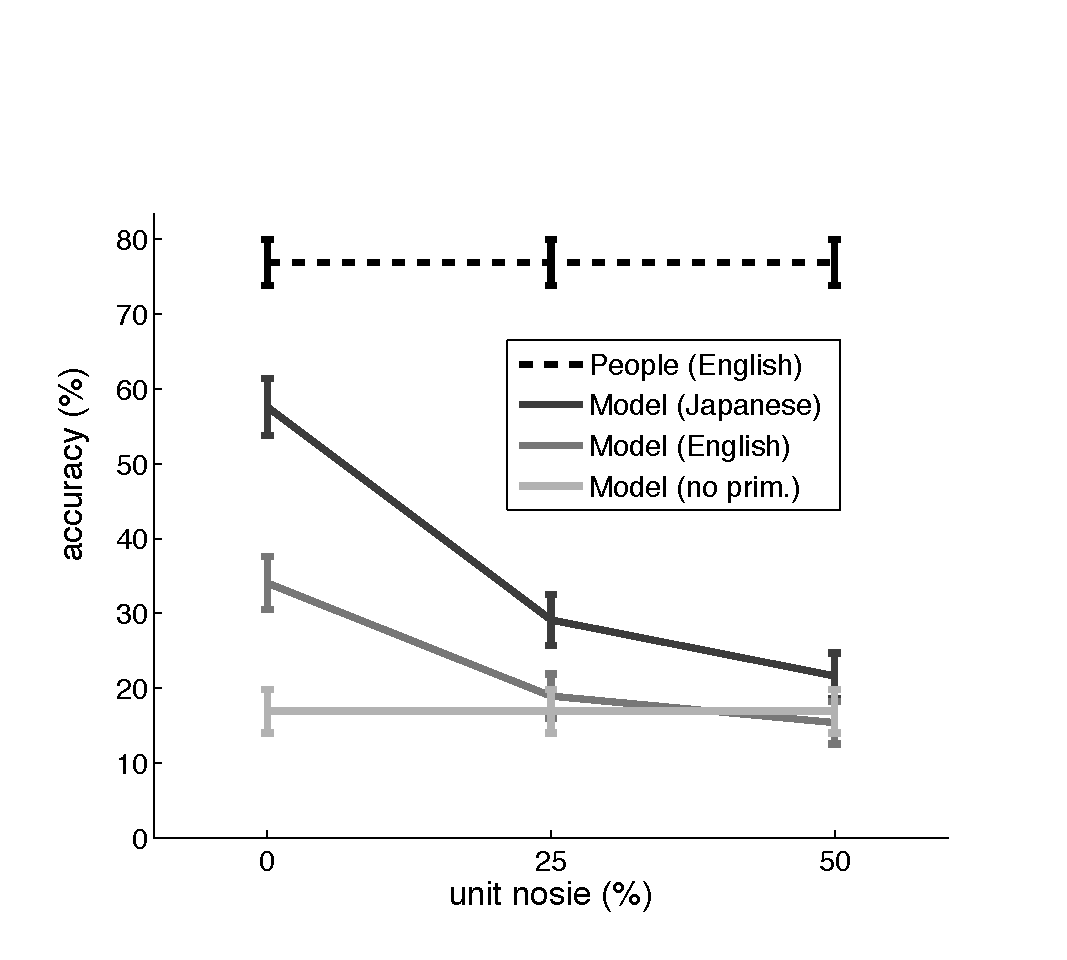
\includegraphics[width=3.25in]{gen_results.pdf}
\caption{Percent of synthesized examples that participants classified into the correct category.}
\label{gen_results}
\end{figure}

\subsection{Replication}
As mentioned, a number of participants in the evaluation task commented on its difficulty. Since the human and machine produced speech were intermixed, and much of the machine speech was intentionally heavily degraded, it is possible that some participants decided it was too difficult to interpret any of the machine speech and thus expended less effort on those trials. This possibility was investigated by running the same trials in a between subjects design, where 45 participants were assigned to one of three conditions: speech generated by people, by the full HBM trained on Japanese, or by the full HBM trained on English. Three participants were removed for knowing some Japanese, and three more were removed by the same guessing criterion as used earlier. The results largely confirmed the earlier numbers: human generated speech scored 80.8\% on average (previously 76.8\%), HBM trained on Japanese scored 60\% (previously 57.6\%), and HBM trained on English scored 27.3\% (previously 34.1\%). 

\section{Discussion}

\begin{itemize}
\item summarize results
\item discussion on what other domains are similar
\item people can't do one-shot learning for all problems, it is only those which have this special structure?
\end{itemize}

\bibliographystyle{apacite}
\setlength{\bibleftmargin}{.125in}
\setlength{\bibindent}{-\bibleftmargin}

\bibliography{library}
\end{document}